\section{Design}
\label{sec:design}

% Around 5 pages about functional aspects of the FeedApp application.
The main purpose of the FeedApp is to deliver a modern web application that offers a seamless and intuitive experience, allowing users to log in, craft their own surveys and cast votes on existing polls.

\subsubsection*{Use cases}
User can: 
\begin{itemize}
\item Register
\item Create polls
\item Vote on polls
\end{itemize}

\begin{figure}[thb]
	\centering
	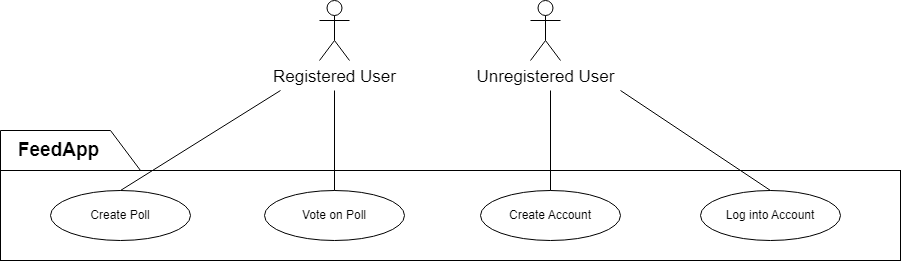
\includegraphics[scale=0.5]{figs/usecase.png}
	\caption{Use Case}
	\label{fig:usecase}
\end{figure}

\subsubsection*{Domain model}
\begin{figure}[thb]
	\centering
	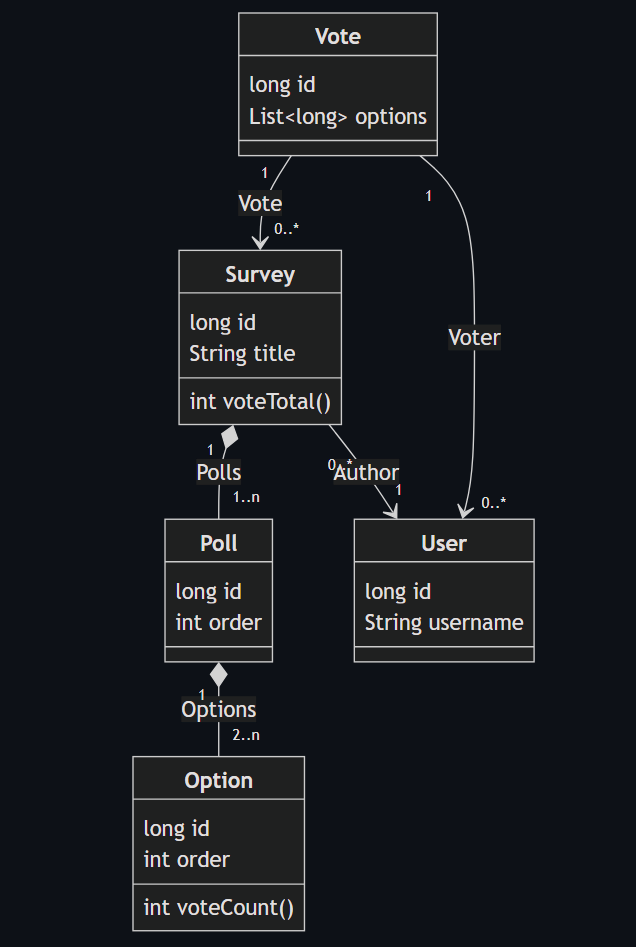
\includegraphics[scale=0.5]{figs/domainmodel.png}
	\caption{The Domain Model.}
	\label{fig:domainmodel}
\end{figure}

\subsubsection*{Architecture}
Blah blah architecture..


%You may have a look at the \href{https://github.com/selabhvl/dat250public/blob/master/projectdescription/README.md}{Examples on GitHub}.

